\begin{center}
\begin{LARGE}
\title{\textbf{Katsiaryna Naumovich}}
\end{LARGE}
\end{center}

\maketitle

\section{Złożoność algorytmów}

\subsection{Teoria złożoności algorytmów}
\begin{justify}
\textbf{Teoria złożoności algorytmów} to dział teorii obliczeń, który zajmuje się badaniem ilości zasobów, takich jak czas, pamięć lub liczba procesorów, potrzebnych do rozwiązania problemów obliczeniowych. Złożoność obliczeniowa algorytmu określa, jak szybko lub jak efektywnie algorytm działa w zależności od rozmiaru danych wejściowych. \par Za twórców tej teorii uważani są \textbf{\textit{Juris Hartmanis}} i \textbf{\textit{Richard Stearns}}. Jako przykłady problemów t.z.o. można podać problem spełnialności, problem najkrótszej ścieżki, problem faktoryzacji oraz wiele innych, o których wiadomo, że są obliczalne. Kwestią obliczalności zajmuje się teoria obliczalności, będąca drugą ważną gałęzią teorii obliczeń.
\end{justify}

\subsection{Złożoność obliczeniowa algorytmu}
\begin{center}
to ilość zasobów komputerowych potrzebnych do jego wykonania:
\end{center}
\begin{itemize}
	\item[--] \textbf{złożoność czasowa}: określa, ile czasu potrzebuje algorytm do wykonania, w zależności od rozmiaru danych wejściowych. Może być wyrażana w najgorszym przypadku (najgorszy czas wykonania), średnim przypadku lub przypadku optymalnym,
	\item[--] \textbf{złożoność pamięciowa}: określa ilość pamięci (RAM) wykorzystywaną przez algorytm w zależności od rozmiaru danych wejściowych.
\end{itemize}

\subsection{Typowe złożoności obliczeniowe}
\begin{enumerate}
	\item \textbf{stała $\Theta(1)$} -- czas wykonania algorytmu jest stały i niezależny od rozmiaru danych wejściowych,
	\item \textbf{logarytmiczna $\Theta(\log n)$} -- czas rośnie logarytmiczne wraz ze wzrostem wielkości danych,
	\item \textbf{liniowa $\Theta(n)$} -- czas działania jest proporcjonalny do rozmiaru danych wejściowych,
	\item \textbf{liniowo-logarytmiczna $\Theta(n \log n)$} -- złożoność jest iloczynem funkcji liniowej i logarytmicznej,
	\item \textbf{kwadratowa $\Theta(n^2)$} -- liczba instrukcji algorytmu rośnie proporcjonalnie do kwadratu rozmiaru danych wejściowych,
	\item \textbf{sześcienna $\Theta(n^3)$} -- liczba instrukcji algorytmu rośnie proporcjonalnie do sześcianu rozmiaru danych wejściowych,
	\item \textbf{wielomianowa $\Theta(n^r + n^{r-1} + \dots + n^1)$} -- liczba instrukcji algorytmu rośnie proporcjonalnie do pewnego wielomianu rozmiaru danych wejściowych,
	\item \textbf{wykładnicza $\Theta(2^n)$} -- czas wykonania rośnie wykładniczo względem rozmiaru danych,
	\item \textbf{silnia $\Theta(n!)$} -- czas wykonania rośnie z szybkością silni względem rozmiaru danych.
\end{enumerate}

Jeśliby założono, że pojedyncza instrukcja wykonuje się jedną nanosekundę (czyli na komputerze działającym z częstotliwością 1 GHz) wtedy czasy wykonania względem rozmiaru danych wyglądałyby następująco:
\begin{table}[htbp]
	\centering
        \renewcommand{\arraystretch}{1.5}
	\begin{tabular}{| c || c | c | c | c | c |}
		\hline
		Rozmiar danych: & 10 & 20 & 50 & 100 & 1000 \\ \hline \hline
		$\log n$ & 
            3,32 ns & 
            4,23 ns & 
            5,64 ns & 
            6,64 ns &
            9,97 ns \\ \hline
		$n$ & 
            10 ns & 
            20 ns & 
            50 ns & 
            100 ns & 
            1 $\mu s$ \\ \hline
		$n \log n$ &
		33,21 ns &
		86,44 ns &
		282,2 ns &
		664,4 ns &
		9,97 $\mu s$ \\ \hline
		$n^2$ &
		100 ns &
		400 ns &
		2,5 $\mu s$ &
		10 $\mu s$ &
		1 ms \\ \hline
		$n^3$ &
		1 $\mu s$ &
		1,05 ms &
		13 dni &
		  $4 \times 10^{13}$ lat &
		$3,4 \times 10^{284}$ lat \\ \hline
		$n!$ &
		3,6 ms &
		77 lat &
		$9,6 \times 10^{44}$ lat &
		$3 \times 10^{141}$ lat & $1,27 \times 10^{2551}$ lat \\ \hline
	\end{tabular}
    \label{tab:algorytmy_tabela}
    \caption{Złożoność obliczeniowa względem rozmiaru danych wejściowych}
\end{table}

Na załączonym wykresie \ref{fig:wykres} widać jak czas wykonania programu rośnie w zależności od wielkości rozwiązywanego problemu.
\begin{figure}[htbp]
    \centering
    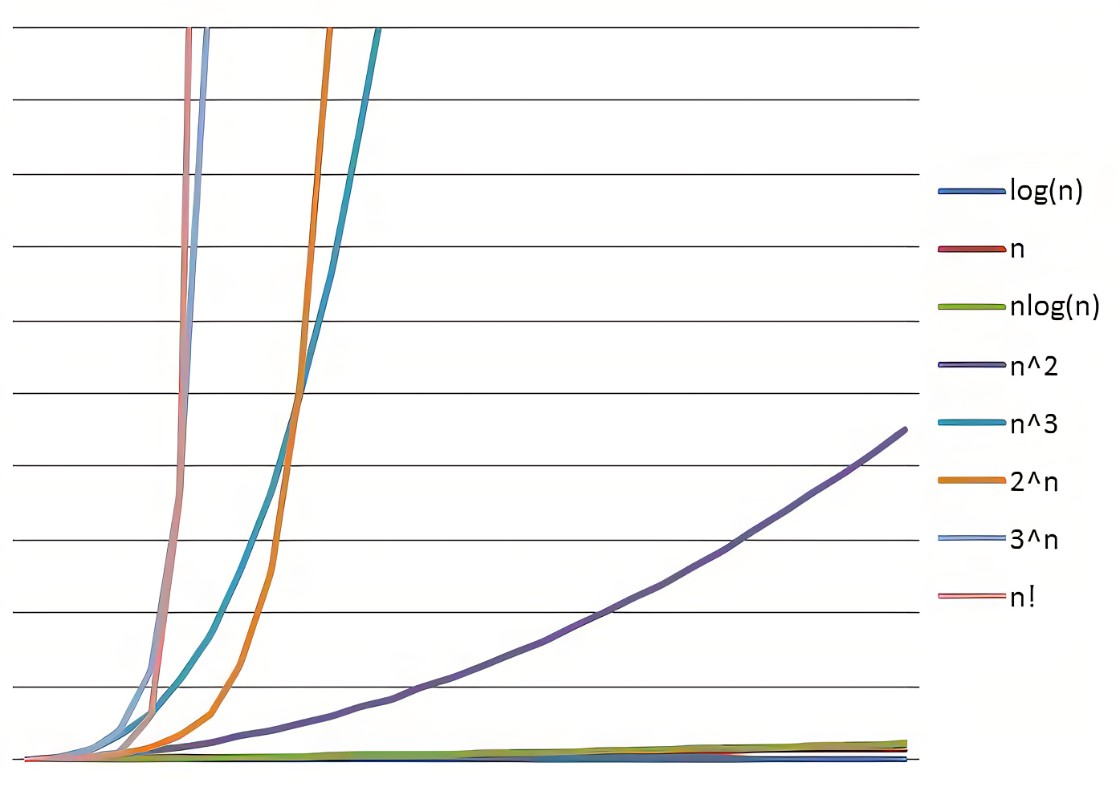
\includegraphics[scale=0.21]{pictures/zlozonosc_obliczeniowa.jpeg}
    \caption{Porównanie złożoności obliczeniowej różnych algorytmów}
    \label{fig:wykres}
\end{figure} 